\section{Durchführung}
\label{sec:Durchführung}

\subsection{Aufbau}

\begin{figure}[h!]
    \centering
    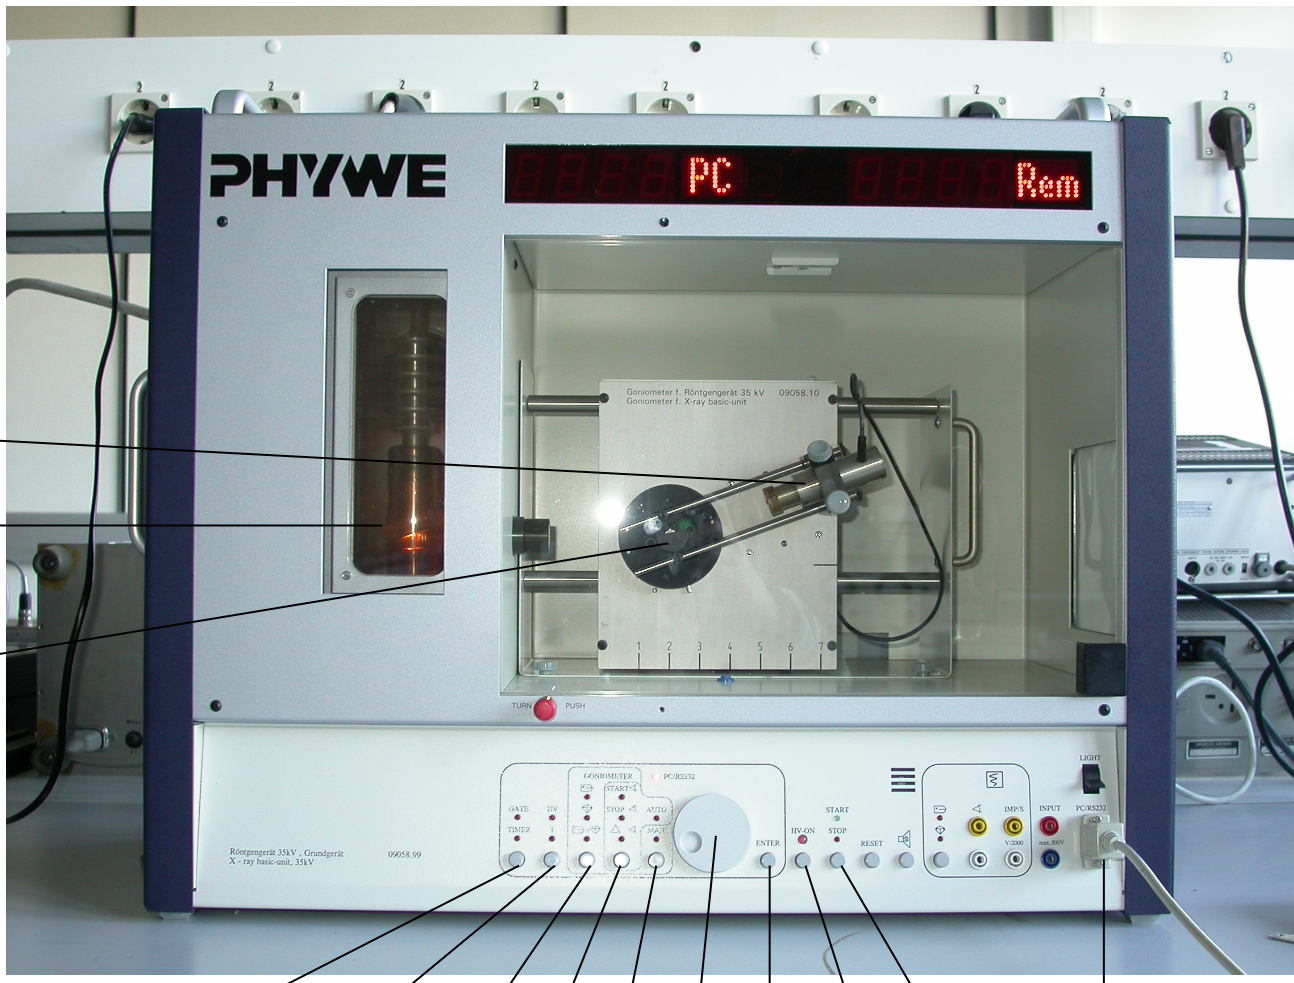
\includegraphics[width=\linewidth]{img/Aufbau_V602.png}
    \caption{Aufbau des Röntgengeräts.\cite{V602}}
    \label{fig:Aufbau}
\end{figure}

Für alle Versuchsteile wird ein Geiger-Müller-Zählrohr, ein LiF-Kristall
und eine Kupfer-Röntgenröhre verwendet. Die Messung wird mithilfe eines an den 
experimentellen Aufbau angeschlossenen Computers durchgeführt.
Über das Messprogramm können die Integrationszeit der Messung, sowie der Winkel des Kristalls und des Zählrohres eingestellt werden.
Die Beschleunigungsspannung wird auf $U_B = \SI{35}{\kilo\volt}$ und der Emissionsstrom auf $I = \SI{1}{\milli\ampere}$ für alle Versuchsteile gestellt.\\
Es können Absorber aus verschiedenen Materialien am Zählrohr angebracht werden.\\

\subsection{Messung}

Im ersten Versuchsteil wird die Bragg-Bedingung überprüft. Der Kristall wir auf einen festen Winkel $Θ = 14°$ eingestellt.
Das Geiger-Müller-Zählrohr wird auf einen Bereich von $α = 26°$ bis $α = 30°$ mit einer Inkrementierung von $Δα = 0.1°$ eingestellt. Die Integrationszeit wird auf $Δt = \SI{5}{\second}$ gesetzt.\\
\\
Im zweiten Versuchsteil wird das charakteristische Emissionsspektrum der Kupfer-Röntgenröhre untersucht. Hierfür wird die Messaparatur in den 2:1 Koppelmodus
gestellt. Das Röntgenspektrum wird in der ersten Beugungsordunung in einem Bereich von $Θ = 4°$ bis $26°$ mit einer Schrittweite von $0.2°$ gemessen. Die Integationszeit jeder Messung beträgt $Δt = \SI{5}{\second}$.\\
Um das Detailspektrum der $K_α$ und $K_β$-Linien zu messen, wird bei gleichbleibender Integrationszeit mit einer Schrittweite von $0.1°$ gemessen. Der Winkelbereich wird so gewählt, dass die beiden Maxima aus der vorgegangenen Messung
genau abgedeckt werden.\\
\\
Im dritten Versuchsteil werden verschiedene Elemente als Absorber vor dem Geiger-Müller-Zählrohr befestigt. Die Integrationszeit wird auf $Δt = \SI{20}{\second}$ eingestellt.
Der Messbereich wird in einem Bereich von $\pm2°$ um den stoffspezifischen Braggwinkel erster Ordnung gewählt. Dieser wird der zweiten Vorbereitungsaufgabe entnommen.\\